%%%%%%%%%%%%%%%%%%%%%%%%%%%%%%%%%%%%%%%%%%%%%%%%%%%
%% LaTeX book template                           %%
%% Author:  Amber Jain (http://amberj.devio.us/) %%
%% License: ISC license                          %%
%%%%%%%%%%%%%%%%%%%%%%%%%%%%%%%%%%%%%%%%%%%%%%%%%%%

\documentclass[a4paper,10pt,twocolumn]{book}

\usepackage[T1]{fontenc}
\usepackage[utf8]{inputenc}
\usepackage{lmodern}
\usepackage{hyperref}
\usepackage{graphicx}
\usepackage[english]{babel}
\usepackage[framemethod=TikZ]{mdframed}
\usepackage{xcolor}
\usepackage{soul}
\usepackage{tkz-euclide}
\usetikzlibrary{calc}
\usepackage[]{algorithm2e}
\usepackage{changepage}
\usepackage{amssymb}
\usepackage{bm}
\usepackage{xcolor}
\usepackage{mathtools}
\usepackage{tcolorbox}
\usepackage{tikz}
\usepackage{tikz-3dplot}
\usepackage{tkz-euclide}
\usepackage{circuitikz}
\usepackage{pgfplots}
\usepackage{subcaption}
\usepackage[inline]{enumitem}\usepackage{geometry}
\geometry{
    a4paper,
    total={170mm,257mm},
    left=15mm,
    right=15mm,
    top=15mm,
    bottom=15mm,
}
\usepackage{multicol}


% \pgfplotsset{width=7cm,compat=1.8}

\usepackage{blindtext}

\usetikzlibrary{positioning}

% EXAMPLES
%% set the counter for your environment
\newcounter{example}
\renewcommand{\theexample}{\thesection.\arabic{example}}

\newcounter{definition}
\renewcommand{\thedefinition}{\thechapter.\arabic{example}}

%% define the style
\mdfdefinestyle{example}{%
    linecolor=red,
    outerlinewidth=0.5pt,
    topline=false,
    bottomline=false,
    % leftline=false,
    rightline=false,
    skipabove=\baselineskip,
    skipbelow=\baselineskip,
    frametitle=\mbox{},
}

\mdfdefinestyle{definition}{%
    linecolor=blue,
    outerlinewidth=0.5pt,
    topline=false,
    bottomline=false,
    rightline=false,
    skipabove=\baselineskip,
    skipbelow=\baselineskip,
    frametitle=\mbox{},
}
%% setup the environments
%%% with number
\newmdenv[%
    style=example,
    settings={\global\refstepcounter{example}},
    frametitlefont={\bfseries {Example}~\theexample\quad},
]{example}

%%% without number (starred version)
\newmdenv[%
    style=example,
    frametitlefont={\bfseries Example~\quad},
]{example*}

%%% without number (starred version)
\newmdenv[%
    style=example,
    frametitlefont={\bfseries {\color{red!70!} Problem}~\quad},
]{problem*}

%%% dwith number
\newmdenv[%
    style=definition,
    settings={\global\refstepcounter{example}},
    frametitlefont={\bfseries {\color{blue!70!} Definition}~\thedefinition\quad},
]{definition}

% BOXES
%% set up the environment
\newmdenv[%
    backgroundcolor=red!8,
    linecolor=red,
    outerlinewidth=1pt,
    roundcorner=5mm,
    skipabove=\baselineskip,
    skipbelow=\baselineskip,
]{myboxed}


\def\mf{\ensuremath\mathbf}
\def\mb{\ensuremath\mathbb}
\def\mc{\ensuremath\mathcal}
\def\lp{\ensuremath\left(}
\def\rp{\ensuremath\right)}
\def\lv{\ensuremath\left\lvert}
\def\rv{\ensuremath\right\rvert}
\def\lV{\ensuremath\left\lVert}
\def\rV{\ensuremath\right\rVert}
\def\lc{\ensuremath\left\{}
\def\rc{\ensuremath\right\}}
\def\ls{\ensuremath\left[}
\def\rs{\ensuremath\right]}
\def\bmx{\ensuremath\begin{bmatrix*}[r]}
\def\emx{\ensuremath\end{bmatrix*}}
\def\bmxc{\ensuremath\begin{bmatrix*}[c]}

\newcommand{\demoex}[2]{\onslide<#1->\begin{color}{black!60} #2 \end{color}}
\newcommand{\demoexc}[3]{\onslide<#1->\begin{color}{#2} #3 \end{color}}
\newcommand{\anim}[3]{\onslide<#1->{\begin{color}{#2!60} #3 \end{color}}}
\newcommand{\ct}[1]{\lp #1\rp}
\newcommand{\dt}[1]{\ls #1\rs}
\newcommand{\cols}[2]{\begin{columns}[#1] #2 \end{columns}}
\newcommand{\col}[2]{\begin{column}{#1} #2 \end{column}}
\newcommand{\eqnwl}[1]{\begin{equation} #1 \end{equation}}
\newcommand{\eqnwol}[1]{\begin{equation*} #1 \end{equation*}}
% \newcommand{\definition}[2]{\vspace{0.25cm}\noindent\textbf{\underline{Definition}}: \textbf{#1}\\\textit{#2}}


\renewcommand{\familydefault}{\sfdefault}

%%%%%%%%%%%%%%%%%%%%%%%%%%%%%%%%%%%%%%%%%%%%%%%%%%%%%%%%%%%%%%%%%%%%%%%%%%%%%%%%
% 'dedication' environment: To add a dedication paragraph at the start of book %
% Source: http://www.tug.org/pipermail/texhax/2010-June/015184.html            %
%%%%%%%%%%%%%%%%%%%%%%%%%%%%%%%%%%%%%%%%%%%%%%%%%%%%%%%%%%%%%%%%%%%%%%%%%%%%%%%%
\newenvironment{dedication}
{
   \cleardoublepage
   \thispagestyle{empty}
   \vspace*{\stretch{1}}
   \hfill\begin{minipage}[t]{0.66\textwidth}
   \raggedright
}
{
   \end{minipage}
   \vspace*{\stretch{3}}
   \clearpage
}

%%%%%%%%%%%%%%%%%%%%%%%%%%%%%%%%%%%%%%%%%%%%%%%%
% Chapter quote at the start of chapter        %
% Source: http://tex.stackexchange.com/a/53380 %
%%%%%%%%%%%%%%%%%%%%%%%%%%%%%%%%%%%%%%%%%%%%%%%%
\makeatletter
\renewcommand{\@chapapp}{}% Not necessary...
\newenvironment{chapquote}[2][2em]
  {\setlength{\@tempdima}{#1}%
   \def\chapquote@author{#2}%
   \parshape 1 \@tempdima \dimexpr\textwidth-2\@tempdima\relax%
   \itshape}
  {\par\normalfont\hfill--\ \chapquote@author\hspace*{\@tempdima}\par\bigskip}
\makeatother

%%%%%%%%%%%%%%%%%%%%%%%%%%%%%%%%%%%%%%%%%%%%%%%%%%%
% First page of book which contains 'stuff' like: %
%  - Book title, subtitle                         %
%  - Book author name                             %
%%%%%%%%%%%%%%%%%%%%%%%%%%%%%%%%%%%%%%%%%%%%%%%%%%%

% Book's title and subtitle
% \title{\Huge \textbf{Linear Systems} \footnote{} \\ \huge Course Notes \footnote\{}}
\title{\Huge \textbf{Linear Systems}\\ \huge Course Notes}
% \title{\Huge \textbf{Linear Systems}}
% Author
% \author{\textsc{Sivakumar Balasubramanian}\thanks{\url{www.example.com}}}
\author{\textsc{Sivakumar Balasubramanian}}

\begin{document}

\frontmatter
\maketitle

%%%%%%%%%%%%%%%%%%%%%%%%%%%%%%%%%%%%%%%%%%%%%%%%%%%%%%%%%%%%%%%
% Add a dedication paragraph to dedicate your book to someone %
%%%%%%%%%%%%%%%%%%%%%%%%%%%%%%%%%%%%%%%%%%%%%%%%%%%%%%%%%%%%%%%
% \begin{dedication}
% Dedicated to Calvin and Hobbes.
% \end{dedication}

%%%%%%%%%%%%%%%%%%%%%%%%%%%%%%%%%%%%%%%%%%%%%%%%%%%%%%%%%%%%%%%%%%%%%%%%
% Auto-generated table of contents, list of figures and list of tables %
%%%%%%%%%%%%%%%%%%%%%%%%%%%%%%%%%%%%%%%%%%%%%%%%%%%%%%%%%%%%%%%%%%%%%%%%
\tableofcontents
% \listoffigures
% \listoftables

\mainmatter

%%%%%%%%%%%
% Preface %
%%%%%%%%%%%
% \chapter*{Preface}
% Lorem ipsum dolor sit amet, consectetur adipiscing elit. Duis risus ante, auctor et pulvinar non, posuere ac lacus. Praesent egestas nisi id metus rhoncus ac lobortis sem hendrerit. Etiam et sapien eget lectus interdum posuere sit amet ac urna.

% \section*{Un-numbered sample section}
% Lorem ipsum dolor sit amet, consectetur adipiscing elit. Duis risus ante, auctor et pulvinar non, posuere ac lacus. Praesent egestas nisi id metus rhoncus ac lobortis sem hendrerit. Etiam et sapien eget lectus interdum posuere sit amet ac urna. Aliquam pellentesque imperdiet erat, eget consectetur felis malesuada quis. Pellentesque sollicitudin, odio sed dapibus eleifend, magna sem luctus turpis.

% \section*{Another sample section}
% Lorem ipsum dolor sit amet, consectetur adipiscing elit. Duis risus ante, auctor et pulvinar non, posuere ac lacus. Praesent egestas nisi id metus rhoncus ac lobortis sem hendrerit. Etiam et sapien eget lectus interdum posuere sit amet ac urna. Aliquam pellentesque imperdiet erat, eget consectetur felis malesuada quis. Pellentesque sollicitudin, odio sed dapibus eleifend, magna sem luctus turpis, id aliquam felis dolor eu diam. Etiam ullamcorper, nunc a accumsan adipiscing, turpis odio bibendum erat, id convallis magna eros nec metus.

% \section*{Structure of book}
% % You might want to add short description about each chapter in this book.
% Each unit will focus on <SOMETHING>.

% \section*{About the companion website}
% The website\footnote{\url{https://github.com/amberj/latex-book-template}} for this file contains:
% \begin{itemize}
%   \item A link to (freely downlodable) latest version of this document.
%   \item Link to download LaTeX source for this document.
%   \item Miscellaneous material (e.g. suggested readings etc).
% \end{itemize}

%%%%%%%%%%%%%%%%%%%%%%%%%%%%%%%%%%%%
% Give credit where credit is due. %
% Say thanks!                      %
%%%%%%%%%%%%%%%%%%%%%%%%%%%%%%%%%%%%
% \section*{Acknowledgements}
% \begin{itemize}
% \item A special word of thanks goes to Professor Don Knuth\footnote{\url{http://www-cs-faculty.stanford.edu/~uno/}} (for \TeX{}) and Leslie Lamport\footnote{\url{http://www.lamport.org/}} (for \LaTeX{}).
% \item I'll also like to thank Gummi\footnote{\url{http://gummi.midnightcoding.org/}} developers and LaTeXila\footnote{\url{http://projects.gnome.org/latexila/}} development team for their awesome \LaTeX{} editors.
% \item I'm deeply indebted my parents, colleagues and friends for their support and encouragement.
% \end{itemize}
% \mbox{}\\
% %\mbox{}\\
% \noindent Amber Jain \\
% \noindent \url{http://amberj.devio.us/}

%%%%%%%%%%%
% Chapets %
%%%%%%%%%%%
% -*- root: ../lsnotes.tex -*-

\chapter{Basics of Linear Algebra and Matrix Theory}

% \begin{chapquote}{Author's name, \textit{Source of this quote}}
% ``This is a quote and I don't know who said this.''
% \end{chapquote}
\section{Vector space}

This chapter mainly consists of a bunch of definitions and concepts about vector spaces that one must be clear about to understand linear algebra. Like most topics in mathematics, or any discipline with a formal structure, the importance of being absolutely clear about the foundational ideas cannot be overstated.

\begin{definition}[frametitle=Vector Space]
A vector space $\mc{V}$ over the field $\mc{F}$ is a non-empty set of elements that is closed under the operations of scalar multiplication and vector addition.
\end{definition}

There are four things involved in a vector space as defined above.
\begin{enumerate}
    \item A non-empty set of elements, where the are called \textbf{vectors}.
    \item A field $\mc{F}$ of scalar that we will be dealing with when working vector spaces. The numbers associated with the elements of the vectors spaces will be from the field $\mc{F}$. We will be mostly dealing with the real $\mb{R}$ or complex $\mb{C}$ scalar fields in this course.  
    \item A vector addition operation denoted by $\mf{v}_1 + \mf{v}_2$, where $\mf{v}_1, \mf{v}_2 \in \mc{V}$.
    \item A scalar multiplication operation denoted by $\alpha \mf{v}_1$ between an element of $\mf{v} \in \mc{V}$ and $\alpha \in \mc{F}$. 
\end{enumerate}
Note: The exact nature of the vector addition and scalar multiplication operations need to be defined depending on the type of vector space we are dealing with. 

Vector spaces generalize the idea of Euclidean (flat) spaces that we are very familiar with from our everyday experience and also most our basic math from school.

The most common example of vector spaces that we will encounter in this course are the n-tuple of numbers, which could be thought of as points in an n-dimensional Euclidean space. Consider the all familiar $xy$-plane shown in Fig. \ref{fig:xyplane}. The set of all points in this plane forms a vector space. Each point in this plane can be represented by 2-tuple of real numbers,
\[ \mb{R}^2 = \lc \bmx x_1 \\ x_2 \emx \bigg\vert \, x_1, x_2 \in \mb{R} \rc  = \lc \ldots \mf{p}_1, \ldots \mf{p}_2, \ldots \rc \]

\noindent The points $\mf{p}_1$, $\mf{p}_2$ shown in Fig. \ref{fig:xyplane} would be somewhere in the set $\mb{R}^2$.

Similarly, the set of all points in $n$-dimensional Euclidean space form a vector space,
\[ \mb{R}^n = \lc \bmxc x_1 \\ x_2 \\ \vdots \\ x_n \emx \bigg\vert \, x_1, x_2, \ldots x_n \in \mb{R} \rc \]

Vector addition between two $n$-tuples $\mf{v}, \mf{w}$ is defined as the sum of the corresponding scalar elements,
\[ \mf{v} + \mf{w} = \bmxc v_1 \\ v_2 \\ \vdots \\ v_n\emx + \bmxc w_1 \\ w_2 \\ \vdots \\ w_n \emx \triangleq \bmxc v_1 + w_1 \\ v_2 + w_2 \\ \vdots \\ v_n + w_n\emx \]

Scalar multiplication of an $n$-tuple by a scalar $\alpha \in \mb{R}$ is defined as,
\[ \alpha \mf{v} = \alpha \bmxc v_1 \\ v_2 \\ \vdots \\ v_n \emx \triangleq \bmxc \alpha v_1 \\ \alpha v_2 \\ \vdots \\ \alpha v_n \emx   \]

\begin{figure}
    \centering
    \resizebox {0.7\columnwidth} {!} {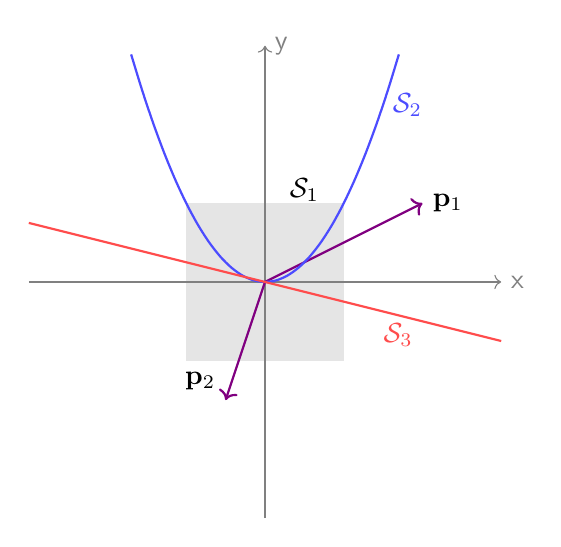
\begin{tikzpicture}[scale=1.0]
    \draw [fill=gray!20!, gray!20!] (-1,-1) rectangle (1,1); 
    \node[black, above] at (0.5, 0.9) {$\mc{S}_1$};
    \draw[thin, gray, ->] (-3, 0)  -> (3, 0) node[right, gray] {x};
    \draw[thin, gray, ->] (0, -3)  -> (0, 3) node[right, gray] {y};
    \draw[thick, violet, ->] (0, 0) -> (2, 1) node[right, black] {$\mf{p}_1$};
    \draw[thick, violet, ->] (0, 0) -> (-0.5, -1.5) node[above left, black] {$\mf{p}_2$};
    \draw[blue!70!, thick] plot[smooth, domain=-1.7:1.7] (\x, {(\x)^2});
    \node[blue!70!, right] at (1.5, 2.25) {$\mc{S}_2$};
    \draw[red!70!, thick] plot[smooth, domain=-3.:3.0] (\x, {-0.25*(\x)});
    \node[red!70!, below left] at (2, -0.4) {$\mc{S}_3$};
    \end{tikzpicture}
    }
    \caption{$xy$-plane.}
    \label{fig:xyplane}
\end{figure}

The elements of the $n$-tuple results from vector addition and scalar multiplication are all real number and thus belong to $\mb{R}^n$. 

The vector addition and scalar multiplication operations associated with a vector space $\mc{V}$,
\begin{enumerate}
    \item $\mf{v} + \mf{w} = \mf{w} + \mf{v}$.
    \item $\mf{u} + \lp \mf{v} + \mf{w} \rp = \lp \mf{u} + \mf{v} \rp + \mf{w}$.
    \item There is a zero element in the vector space $\mc{V}$, $\mf{0} \in \mc{V}$, such that $\mf{v} + \mf{0} = \mf{v}$.
    \item For every $\mf{v} \in \mc{V}$, there is an element $-\mf{v}$, such that $\mf{v} + \lp -\mf{v}\rp = \mf{0}$.
    \item $\lp \alpha \beta \rp \mf{v} = \alpha \lp \beta \mf{v}\rp$, $\forall \alpha, \beta \in \mc{F}$ and $\forall \mf{v} \in \mc{V}$.
    \item $\alpha \lp \mf{v} + \mf{w} \rp  = \alpha \mf{v} + \alpha \mf{w}$, $\forall \alpha \in \mc{F}$ and $\forall \mf{v},\mf{w} \in \mc{V}$.
    \item $\lp \alpha + \beta \rp \mf{v} = \alpha \mf{v} + \beta \mf{v}$, $\forall \alpha, \beta \in \mc{F}$ and $\forall \mf{v} \in \mc{V}$.
    \item $1 \mf{v} = \mf{v}, \, \forall \mf{v} \in \mc{V}$.
\end{enumerate}

\section{Subspace}
Consider a vector space $\mc{V}$\footnote{Whenever you hear see the term `vector space', you must train yourself to immediately think of the the Def. 1.1}. Let us now consider $\mc{S}$, a subset of $\mc{V}$, i.e. $\mc{S} \subseteq \mc{V}$. This means that if $x \in \mc{S}$ then $x \in \mc{V}$. A subset of $\mc{V}$ qualifies to a subspace of $\mc{V}$ only if $\mc{S}$ itself is a vector space.

\begin{definition}[frametitle=Subspace]
Let $\mc{S}$ be a non-empty subset of a vector space $\mc{V}$ over the field $\mc{F}$. $\mc{S}$ is a subspace over the same field $\mc{F}$ with the same vector addition and scalar multiplication operations as $\mc{V}$, if and only if $\mc{S}$ is closed under the vector addition and scalar multiplication operations.
\begin{align*}
\mf{x}, \mf{y} \in \mc{S} &\implies \mf{x} + \mf{y} \in \mc{S}\\
\mf{x} \in \mc{S} \text{ and } \alpha \in \mc{F} &\implies \alpha \mf{x} \in \mc{S}
\end{align*}
\end{definition}

Let us look at some examples to get a good grasp of what subspaces are. $\mc{V} = \mb{R}^2$ is the parent vector space. 
\[ \mc{V} = \mb{R}^2 = \lc \bmxc x_1 \\ x_2\emx \bigg\vert \, x_1, x_2 \in \mb{R} \rc\]

The following are some of non-empty subsets of $\mb{R}^2$ (shown in Fig. \ref{fig:xyplane}, but not all of them are subspaces. 
\begin{enumerate}
    \item $\mc{S}_1 = \lc \bmxc x_1\\ x_2 \emx \bigg\vert \, \lv x_1 \rv \leq 1, \lv x_2 \rv \leq 1\rc$. This is the set of all points in the gray square shown in Fig. \ref{fig:xyplane}.

    This is \textbf{\underline{not}} a subspace of $\mc{V}$. Because, it is not closed under scalar multiplication or vector addition. For example, $\mf{v}_1 =  \bmxc 1 \\ 1\emx, \mf{v}_2 = \bmxc -1 \\ 1\emx \in \mc{S}_1$, but $\mf{v}_1 + \mf{v}_2 = \bmxc 0 \\ 2\emx \notin \mc{S}_1$.

    \item $\mc{S}_2 = \lc \bmxc x_1\\ x_2 \emx \bigg\vert \, x_1 \in \mb{R}, \, x_2 = x_1^2 \rc$. This is the set of all points on the blue colored parabola in Fig. \ref{fig:xyplane}.

    This is also \textbf{\underline{not}} a subspace of $\mc{V}$, as it is not closed under scalar multiplication or vector addition. Let, $\mf{v}_1 =  \bmxc 1 \\ 1\emx \in \mc{S}_2$, but $2\mf{v}_1 = \bmxc 2 \\ 2\emx \notin \mc{S}_2$.

    \item $\mc{S}_3 = \lc \bmxc x_1\\ x_2 \emx \bigg\vert \, x_1 \in \mb{R}, \, x_2 = \beta x_1, \beta \in \mb{R} \rc$. This is the set of all points on the red line passing through the origin in Fig. \ref{fig:xyplane}.

    This is a subspace of $\mc{V}$; it is closed under scalar multiplication or vector addition. 

    Let $\mf{v} = \bmxc v_1 \\ \beta v_1\emx$ and $\mf{w} = \bmxc w_1 \\ \beta w_1\emx$. Then, $\alpha \mf{v} = \bmxc \alpha v_1 \\ \alpha \beta v_1\emx = \bmxc \alpha v_1 \\ \beta \lp \alpha v_1 \rp\emx \in \mc{S}_3$.

    And, $\mf{v} + \mf{w} = \bmxc v_1 \\ \beta v_1\emx + \bmxc w_1 \\ \beta w_1\emx = \bmxc v_1 + w_1\\ \beta v_1 + \beta w_1\emx = \bmxc v_1 + w_1\\ \beta \lp v_1 + w_1 \rp\emx \in \mc{S}_3$.
\end{enumerate}

\begin{problem*}[frametitle=Subspaces]
Which of the following subsets are subspaces of $\mb{R}^2$?
\begin{enumerate}
    \item $\lc \alpha \mf{p} \,\, \vert \,\, \mf{p} \in \mb{R}^2, \alpha = \mb{R} \rc$.
    \item $\lc \alpha \mf{p} + \mf{q} \,\, \vert \,\, \mf{p}, \mf{q} \in \mb{R}^2, \alpha = \mb{R} \rc$.
    \item $\lc \mf{p} = \bmxc p_1 \\ p_2\emx \,\, \bigg\vert \,\, \mf{p} \in \mb{R}^2, \, p_1^2 + p_2^2 = 1 \rc$.
    \item $\lc \mf{p} = \bmxc p_1 \\ p_2\emx \,\, \bigg\vert \,\, \mf{p} \in \mb{R}^2, \, p_1^2 + p_2^2 = 0 \rc$.
\end{enumerate}
\end{problem*}

\section{Span of a set of vectors}
Consider a set of vectors $\mc{S} = \lc \mf{v}_1, \mf{v}_2, \ldots \mf{v}_n\rc, \, \mf{v}_i \in \mc{V}, \, 1 \leq i \leq n$, where $\mc{V}$ is a vector space over the field $\mc{F}$\footnote{From now on, we will assume that a given vector space is over the field $\mf{F}$, unless specified otherwise.}. A linear combination of the elements of $\mc{S}$ is a vector $\mf{u} \in \mc{V}$ defined as the following,
\[ \mf{u} = \sum_{i=1}^{n}\alpha_i\mf{v}_i, \, \alpha_i \in \mc{F}, \, \mf{v}_i \in \mc{S} \]

\begin{definition}[frametitle=Span of set of vectors]
The span of a set of vectors $S = \lc \mf{v}_1, \mf{v}_2, \ldots \mf{v}_n\rc$ is defined as the set of all linear combinations of a the elements of $\mc{S}$, i.e.
\[ span\lp \mc{S} \rp = \lc \sum_{i=1}^n\alpha_i\mf{v}_i \bigg\vert \alpha \in \mc{F} \rc \]
\end{definition}

What can we say about $span\lp \mc{S}\rp$? Is it a subset of $\mc{V}$? Is it a subspace of $\mc{V}$? It turns out that the span of a set of vector does form a subspace of $\mc{V}$. It is left as an exercise for the reader to prove this.

The subspace $span\lp\mc{S}\rp$ is called the subspace spanned by $\mc{S}$, or $\mc{S}$ is said to span the subspace $span\lp \mc{S}\rp$. $\mc{S}$ is also called the spanning set of $span\lp \mc{S}\rp$.

\begin{problem*}[frametitle=Span of a set of vectors]
\begin{enumerate}
    \item Consider a set of vectors $\mc{S} = \lc \mf{v}_1, \mf{v}_2, \ldots \mf{v}_n\rc, \, \mf{v}_i \in \mc{V}, \, 1 \leq i \leq n$, where $\mc{V}$ is a vector space. Prove that a linear combination of the vectors of $\mc{S}$ belong to $\mc{V}$.
    \item Prove that the span of a set $\mc{S}$ is a subspace of $\mc{V}$.
\end{enumerate}
\end{problem*}

\section{Linear independence}
Like the span, linear independence (LI) is also a concept associated with a set of vectors $\mc{S} = \lc \mf{v}_1, \mf{v}_2, \ldots \mf{v}_n\rc, \, \mf{v}_i \in \mc{V}, \, 1 \leq i \leq n$ where $\mc{V}$ is a vector space. LI tells us if one or more vectors in $\mc{S}$ is in the subspace spanned by other vectors in $\mc{S}$ (or if one or more vectors is a linear combination of the other vectors in $\mc{S}$). 

\begin{definition}[frametitle=Linear Independene]
A set of vectors $\mc{S} = \lc \mf{v}_1, \mf{v}_2, \ldots \mf{v}_n\rc$ is a linearly independent set if and only if,
\[ \sum_{i=1}^n \alpha_i\mf{v}_i = 0 \implies \alpha_i = 0, \forall i\]

\noindent The set is linearly dependent if at least one of the $\alpha_i \neq 0$. 
\end{definition}

\section{Basis and dimension of a vector space}
Vector spaces can consist of infinite number of elements. The special structure of vector spaces (closure under scalar multiplication and addition) allows us to generate all elements of a vector space using only a finite number of elements from that vector space\footnote{This is only valid for finite dimensional vector space, and in this course we will only talk about finite dimensional vector space.}. We have seen this earlier: a spanning set $\mc{S}$ (consisting of a finite number of elements) can be used to generate all elements in the subspace $span\lp \mc{S}\rp$. 

Consider a set $\mc{S} = \lc \mf{v}_1, \mf{v}_2, \ldots \mf{v}_n\rc, \, \mf{v}_i \in \mc{V}, \, 1 \leq i \leq n$, a subset of the vector space $\mc{V}$, whose elements can be used to generate every element of $\mc{V}$ through a linear combination, i.e. $\forall \mf{x} \in \mc{V}, \exists \alpha_i \in \mc{F}, 1 \leq i \leq n$ such that , 
\[ \mf{x} = \sum_{i=1}^n\alpha_i \mf{v}_i \]

A basis of a vector space $\mc{V}$ is a set with the least number of elements, which can be used to generate all elements of $\mc{V}$. Thus, a basis is a set with the sufficient of elements from $\mc{V}$ that are necessary to generate all elements of $\mc{V}$. 

\begin{definition}[frametitle=Basis of a vector space]
A linearly independent spanning set of a vector space $\mc{V}$ is called a basis of $\mc{V}$.
\end{definition}

There can be an infinite number of basis for a vector space $\mc{V}$. Apart from the all of them sharing a property of being linearly independent spanning sets of $\mc{V}$, there share another common property. They all have the same number of elements. This number is called the dimension of the vector space $\mc{V}$.

\begin{definition}[frametitle=Dimension of a vector space]
The dimension of a vector space $\text{dim} \mc{V}$ is the number of elements of a basis the basis of $\mc{V}$.
\end{definition} 

One of the advantages of a basis is that there is a unique representation, in terms of the elements of the basis, for every element from the span of the basis. Consider a basis $\mc{S} = \lc \mf{v}_i \rc_{i=1}^n$ of the vetor space $\mc{V}$, there $\forall \mf{x} \in \mc{V}$, we can write 
\[ \mf{x} = \sum_{i=1}^n \alpha_i\mf{v}_i \]
where the $\alpha_i$ are unique. There is only one way to write $\mf{x}$ as a linear combnation of the elements $\mf{v}_i$ of the basis $\mc{S}$.

\begin{problem*}[frametitle=Basis and representation of vectors]
Consider linear dependent set of vector $\mc{W} = \lc \mf{w}_i \rc_{i=1}^n$. Prove that there there is not unqiue way to represent a vector $\mf{x} \in span\lp \mc{W} \rp$ in terms of the elements of $\mc{W}$.
\end{problem*}

\begin{figure}[h!]
    \centering
    \resizebox {0.35\columnwidth} {!} {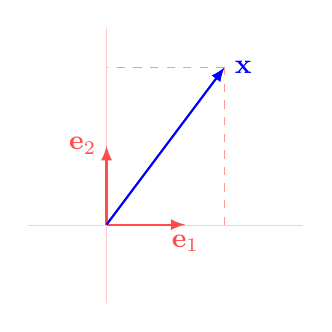
\begin{tikzpicture}[scale=1.0]
    \draw[ultra thin, red!20!, -] (-1, 0)  -> (2.5, 0);
    \draw[ultra thin, red!20!, -] (0, -1)  -> (0, 2.5);
    \draw[thick, red!70!, -latex] (0, 0) -> (1, 0) node[below] {$\mf{e}_1$};
    \draw[thick, red!70!, -latex] (0, 0) -> (0, 1) node[left] {$\mf{e}_2$};
    \draw[thick, blue, -latex] (0, 0) -> (1.5, 2) node[right] {$\mf{x}$};
    \draw[thin, red!40!, dashed] (1.5, 2) -- (1.5, 0);
    \draw[thin, red!40!, dashed] (1.5, 2) -- (0, 2);
    \end{tikzpicture}
    }
    \resizebox {0.35\columnwidth} {!} {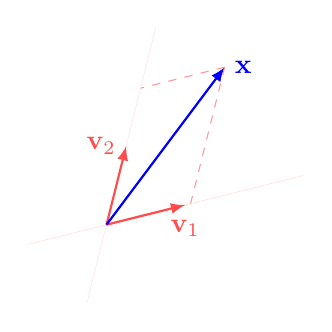
\begin{tikzpicture}[scale=1.0]
    \draw[ultra thin, red!20!, -] (-1, -0.25)  -> (2.5, 0.625);
    \draw[ultra thin, red!20!, -] (-0.25, -1.0)  -> (0.625, 2.5);
    \draw[thick, red!70!, -latex] (0, 0) -> (1, 0.25) node[yshift=-0.3cm] {$\mf{v}_1$};
    \draw[thick, red!70!, -latex] (0, 0) -> (0.25, 1) node[left] {$\mf{v}_2$};
    \draw[thick, blue, -latex] (0, 0) -> (1.5, 2) node[right] {$\mf{x}$};
    \draw[thin, red!40!, dashed] (1.5, 2) -- (16/15, 4/15);
    \draw[thin, red!40!, dashed] (1.5, 2) -- (6.5/15, 26/15);
    \end{tikzpicture}
    }\\
    \resizebox {0.40\columnwidth} {!} {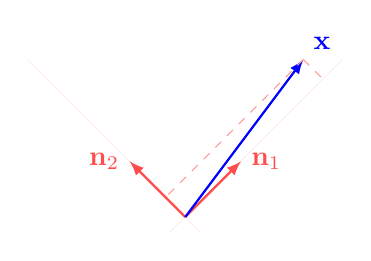
\begin{tikzpicture}[scale=1.0]
    \draw[ultra thin, red!20!, -] (-0.2, -0.2)  -> (2, 2);
    \draw[ultra thin, red!20!, -] (-2, 2)  -> (0.2, -0.2);
    \draw[thick, red!70!, -latex] (0, 0) -> (0.707, 0.707) node[right] {$\mf{n}_1$};
    \draw[thick, red!70!, -latex] (0, 0) -> (-0.707, 0.707) node[left] {$\mf{n}_2$};
    \draw[thick, blue, -latex] (0, 0) -> (1.5, 2) node[above right] {$\mf{x}$};
    \draw[thin, red!40!, dashed] (1.5, 2) -- (1.75, 1.75);
    \draw[thin, red!40!, dashed] (1.5, 2) -- (-0.25, 0.25);
    \end{tikzpicture}
    }
    \caption{$\mb{R}^2$ vector space}
    \label{fig:r2basis}
\end{figure}

\section{Orthonormal basis}
Although there can be infinitely many basis for a vector space, some basis are natural or more easy to work with. For example, consider the unit vectors, 
\[ \mf{e}_1 = \bmxc 1 \\0 \\0 \\ \vdots \\ 0\emx, \, \mf{e}_2 = \bmxc 0 \\1 \\0 \\ \vdots \\ 0\emx, \, \mf{e}_3 = \bmxc 0 \\0 \\ 1 \\ \vdots \\ 0\emx \ldots \mf{e}_n = \bmxc 0 \\0 \\0 \\ \vdots \\ 1\emx \]

The set of unit vectors $\mc{E} = \lc \mf{e}_i \rc_{i=1}^n$ form a basis for $\mb{R}^n$. It is easy to see how any vector $\mf{x} = \bmx x_1\\ x_2 \\ \vdots \\ x_n\emx \in \mb{R}^n$ can be represented in the basis $\mc{E}$.
\[ \mf{x} = \bmx x_1\\ x_2 \\ x_3 \\ \vdots \\ x_n\emx = \sum_{i-1}^n x_i\mf{e}_i \]
With the basis $\mc{E}$ it is easy to find out the scalars that one needs to use to represent a vector $\mf{x}$ as a linear combination of the elements of $\mc{E}$. For other abitrary basis it is not easy to find out the exact scalars that go in the linear combination (e.g. the second plot shown in Fig. \ref{fig:r2basis}). However, when a basis is orthonormal, then finding the scalars in the linear comination are relatively easy. An orthonormal basis $\mc{N} = \lc\mf{n}_i\rc_{i=1}^n$ is a basis with the following properties,
\[ \mf{n}_i^T\mf{n}_j = \begin{cases} 1 & i = j \\ 0 & i \neq j \end{cases} \]
All vectors have unit length (-2-norm), and mutually orthogonal. Suppose that the representation of $\mf{x}$ in the basis $\mc{N}$ is given by the following,
\[ \mf{x} = \sum_{i=1}^{n} \alpha_i \mf{n}_i, \quad \alpha_i = \mf{n}_i^T\mf{x} \]

\begin{problem*}
Prove the for an orthonormal basis $\mc{N} = \lc \mf{n}_i \rc_{i=1}^n$ of $\mb{R}^n$, any vector $\mf{x} \in \mb{R}^n$ can be written as,
\[ \mf{x} = \sum_{i=1}^n \lp \mf{n}_i^T\mf{x} \rp\mf{n}_i\]
\end{problem*}

\section{Matrix Multiplication}
Consider two matrices $\mf{A} \in \mb{R}^{m \times p}$ and $\mf{B} \in \mb{R}^{p \times n}$, the product of these two matrices is $\mf{C} \in \mb{R}^{m \times n}$,
\[ \mf{C} = \mf{A}\mf{B} \]
where, the $ij^{th}$ element of $\mf{C}$ is given by,
\[ c_{ij} = \sum_{k=1}^p a_{ik}b_{kj} \]

There are four different ways to make sense of the above equation,
\begin{enumerate}
    \item \textbf{Column view}. The columns of $\mf{C}$ are equal to the linear combination of the columns of $\mf{A}$, and the scalars in the linear combination come from the rows of the corresponding column of $\mf{B}$.
    \[ i^{th} \text{ column of } \mf{C} = \mf{c}_i = \sum_{k=1}^p b_{ik}\mf{a}_k \]

    \item \textbf{Row view}. The rows of $\mf{C}$ are equal to the linear combination of the rows of $\mf{B}$, and the scalars in the linear combination come from the columns of the corresponding row of $\mf{A}$.
    \[ i^{th} \text{ column of } \mf{C} = \tilde{\mf{c}}_i^T = \sum_{k=1}^p a_{ki}\tilde{\mf{b}}_k^T \]

    \item \textbf{Inner product view}. The $ij^{th}$ element of $\mf{C}$ is given by the inner product of the $i^{th}$ row of $\mf{A}$ and the $j^{th}$ columns of $\mf{B}$.
    \[  c_{ij} = \tilde{\mf{a}}_i^T\mf{b}_j \]

    \item \textbf{Outer product view}. The matrix $\mf{C}$ can be written as the sum of $p$ rank-1 matrices\footnote{Matrix whose rank is 1.} $\mf{a}_k\tilde{\mf{b}}_k^T, \, 1 \leq k \leq p$.
    \[ \mf{C} = \sum_{k=1}^p \mf{a}_k\tilde{\mf{b}}_k^T \]
\end{enumerate}

\section{Linear Equations $\mf{y} = \mf{A}\mf{x}$}
Linear equations of the following form are encountered in numerous application across disciplines,
\[ \begin{split}
a_{11}x_1 + a_{12}x_2 \ldots + a_{1n}x_n & = b_1 \\
a_{21}x_1 + a_{22}x_2 \ldots + a_{2n}x_n & = b_2 \\
a_{31}x_1 + a_{32}x_2 \ldots + a_{3n}x_n & = b_3 \\
\vdots \\
a_{m1}x_1 + a_{m2}x_2 \ldots + a_{mn}x_n & = b_m
\end{split} \]
There are $m$ equations and $n$ unknowns. The above equations can be more compactly represented using the matrix notation,
\[ \mf{y} = \mf{A}\mf{x}, \quad \mf{x} \in \mb{R}^n, \mf{y} \in \mb{R}^m, \mf{A} \in \mb{R}^{m \times n} \]
$\mf{A}$ and $\mf{y}$ are known and $\mf{x}$ is to be determined.

Linear equations play an important role in engineering as many engineering problems can be mathematically approximated to have a linear structure.

We can broadly classify a vast majority of applications of linear equations into two categories: \textbf{Control problem} and \textbf{Estimation problem}.

\begin{itemize}
    \item \textbf{Control Problem}. Control problems deal with linear systems with a set of inputs and outputs (Fig. \ref{fig:controlprob}), and our goal is to control the output behavior of the system by appropriately choosing the system inputs. The system has $n$ scalar inputs $\mf{x} = \bmxc x_1\\ x_2 \\ \vdots \\ x_n\emx \in \mb{R}^n$ that we can freely choose, and it has $m$ scalar outputs $\mf{y} = \bmxc y_1\\ y_2 \\ \vdots \\ y_m\emx \in \mb{R}^m$. The matrix $\mf{A}$ contains information about the physics of the system relating the system inputs to the the system outputs   
    \[ \mf{y} = \mf{A}\mf{x} \]
    \begin{figure}[h!]
        \centering
        \resizebox {0.7\columnwidth} {!} {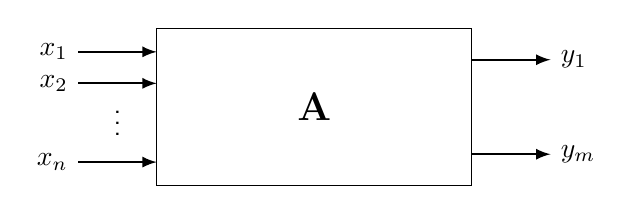
\begin{tikzpicture}[scale=1.0]
        \draw [black] (-2,-1) rectangle (2,1);
        \draw[thick, -latex] (-3.0, 0.7) node[left] {$x_1$} -- (-2, 0.7);
        \draw[thick, -latex] (-3.0, 0.3) node[left] {$x_2$} -- (-2, 0.3);
        \draw[thick, -latex] (-3.0, -0.7) node[left] {$x_n$} -- (-2, -0.7);
        \node[yshift=0.1cm] at (-2.5, -0.2) {$\vdots$};
        \draw[thick, -latex] (2.0, 0.6) -- (3, 0.6) node[right] {$y_1$};
        \draw[thick, -latex] (2.0, -0.6) -- (3, -0.6) node[right] {$y_m$};
        \node at (0, 0) {\Large $\mf{A}$};
        \end{tikzpicture}
        }
        \caption{Control Problem}
        \label{fig:controlprob}
    \end{figure}

    The columns of $\mf{A}$ show how all the $m$ outputs of the system are affected by the $n$ individual inputs, i.e. the $i^{th}$ column is the amount by which the output vector $\mf{y}$ changes due to a unit change in $x_i$. 
    \[ \mf{y} = \ldots + x_i \mf{a}_i + \ldots \]

    The rows of $\mf{A}$ tell us how the all the $n$ input of the system affect a particular output, i.e. the $i^{th}$ row of $\mf{A}$ tell us the complete story about how the different inputs affect the $i^{th}$ output.
    \[ y_i = \tilde{\mf{a}}_i^T\mf{x} \]

    \setcounter{example}{0}
    \begin{example}[frametitle=Applying a force on an object through a multi-joint system]\label{ex:control}
    Assume that one a person is trying to apply a force on a wall using his/her arm consisting of three joints (shoulder, elbow and wrist), as shown in Fig. \ref{fig:controlprob}.

    The force $\mf{f} = \bmxc f_x \\ f_y\emx$ applied on the wall can be controlled through the torque applied at the three joints $\bm{\tau}=\bmxc \tau_S \\ \tau_E \\ \tau_W \emx$. The relationship between the torque and the endpoint force are linearly related for a fixed shoulder, elbow and wrist angle.
    \[ \mf{f} = \bmxc f_x \\ f_y\emx = \bmxc j_{11} & j_{12} & j_{13}\\ j_{21} & j_{22} & j_{23}\emx \bmxc \tau_S \\ \tau_E \\ \tau_W\emx = \mf{J}\bm{\tau} \]
    \end{example}

    \begin{figure}[h!]
    \centering
    \resizebox {0.3\columnwidth} {!} {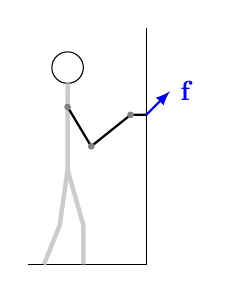
\begin{tikzpicture}[scale=1.0]
    \draw[thin, -] (-2.0, 0) -- (-0.5, 0) -- (-0.5, 3);
    \draw (-1.5, 2.5) circle (0.2);
    \draw[ultra thick, gray!40!] (-1.5, 2.3) -- (-1.5, 1.2) -- (-1.6, 0.5) -- (-1.8, 0);
    \draw[ultra thick, gray!40!] (-1.5, 1.2) -- (-1.3, 0.5) -- (-1.3, 0);
    \draw[thick, black] (-1.5, 2.0) -- (-1.2, 1.5) -- (-0.7, 1.9) -- (-0.5, 1.9);
    \draw[fill=gray, gray] (-1.5, 2.0) circle (0.035);
    \draw[fill=gray, gray] (-1.2, 1.5) circle (0.035);
    \draw[fill=gray, gray] (-0.7, 1.9) circle (0.035);
    \draw[thick, blue, -latex] (-0.5, 1.9) -- (-0.2, 2.2) node[above, right] {$\mf{f}$};
    \end{tikzpicture}
    }
    \resizebox {0.6\columnwidth} {!} {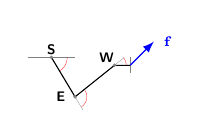
\begin{tikzpicture}[scale=1.0]
    \draw[black] (-1.5, 2.0) -- (-1.2, 1.5) -- (-0.7, 1.9) -- (-0.5, 1.9);
    \draw[ultra thin, gray] (-1.8, 2.0) -- (-1.2, 2.0);
    \draw [ultra thin, red, domain=-57:0] plot ({-1.5 + 0.2*cos(\x)}, {2.0 + 0.2*sin(\x)});
    \node[yshift=0.1cm] at (-1.5, 2.0) {\tiny \textbf{S}};
    \draw[ultra thin, gray] (-1.2, 1.5) -- ++(0.1, -0.1667);
    \draw [ultra thin, red, domain=-57:35] plot ({-1.2 + 0.15*cos(\x)}, {1.5 + 0.15*sin(\x)});
    \node[left] at (-1.2, 1.5) {\tiny \textbf{E}};
    \draw[ultra thin, gray] (-0.7, 1.9) -- ++(0.125, 0.1);
    \draw [ultra thin, red, domain=0:40] plot ({-0.7 + 0.15*cos(\x)}, {1.9 + 0.15*sin(\x)});
    \node[xshift=-0.1cm, yshift=0.1cm] at (-0.7, 1.9) {\tiny \textbf{W}};
    \draw[ultra thin, gray] (-0.5, 1.8) -- ++(0.0, 0.2);
    \draw[blue, -latex] (-0.5, 1.9) -- (-0.2, 2.2) node[above, right] {\tiny $\mf{f}$};
    \draw[fill=gray, gray] (-1.5, 2.0) circle (0.015);
    \draw[fill=gray, gray] (-1.2, 1.5) circle (0.015);
    \draw[fill=gray, gray] (-0.7, 1.9) circle (0.015);
    \end{tikzpicture}
    }
    \caption{Applying a force with the arm.}
    \label{fig:armforce}
    \end{figure}

    \item \textbf{Estimation problem}. Estimation problems deal with  determining unknown parameters or inputs associated with a system using measurements from the system $\mf{y}$ and knowledge of how the system parameters/inputs affect these measurements $\mf{A}$. Assuming a linear relationship between the measurements and the system inputs/parameters, we have
    \[ \mf{y} = \mf{A}\mf{x} \]
    \begin{example}[frametitle=Estimating Mass of an Object]\label{ex:est}
    Consider an object on of mass $m$ on a frictionless surface (Fig. \ref{fig:estmass}). We are interested in determining the system's mass $m$. At any given time $t$, we can apply any desired force $f\ct{t}$ to the system, and measure the system's position $x\ct{t}$, velocity $\dot{x}\ct{t}$ and acceleration $\ddot{x}\ct{t}$. We carry out a controller experiment starting at time $t=0$, where we start the system at rest $\dot{x}\ct{0} = \ddot{x}\ct{0} = 0$ and at position $x\ct{0}=0$; the was not force acting before the start of the experiment $f\ct{t} = 0, \, t < 0$. We apply a constant force $f$ on the system, and measure its position, velocity and acceleration, 1 sec after the application of the force, i.e. we measure $x\ct{1}, \dot{x}\ct{1}, \ddot{x}\ct{1}$. From classical mechanics we know, 
    \[ \mf{x} = \bmxc x\ct{1} \\ \dot{x}\ct{1} \\ \ddot{x}\ct{1} \emx = \bmxc 0.5f \\ f \\ 1 \emx \bmxc \frac{1}{m}\emx = \mf{A}\mf{w} \]

    If we had repeated the experiment $n$ times, then we could combine data from all the experiments and express the measurements with the system parameter $m$ as the following,
    \[ \mf{x} = \bmxc \mf{x}_1 \\ \mf{x}_2 \\ \vdots \\ \mf{x}_n \emx = \bmxc \mf{A}_1 \\ \mf{A}_2 \\ \vdots \\ \mf{A}_n \emx \bmxc \frac{1}{m} \emx \]
    where $\mf{x}_i = \bmxc x_i\ct{1} & \dot{x}_i\ct{1} & \ddot{x}_i\ct{1} \emx^T$ are the measurements from experiment $i$ where a constant force $f_i$ was applied.

    \end{example}

    \begin{figure}[h!]
    \centering
    \resizebox {0.6\columnwidth} {!} {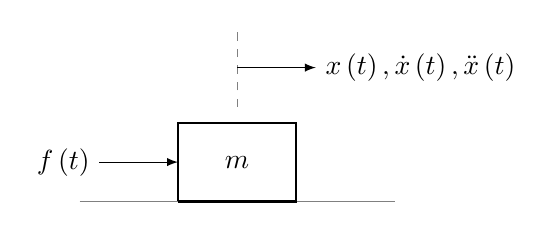
\begin{tikzpicture}[scale=1.0]
    \draw[thin, gray] (-2, 0) -- (2, 0);
    \draw[thick, black] (-0.75, 0) -- (0.75, 0) -- (0.75, 1.0) -- (-0.75, 1.0) -- (-0.75, 0);
    \node[black] at (0, 0.5) {$m$};
    \draw[black, -latex] (-1.75, 0.5) node[left] {$f\ct{t}$} -- (-0.75, 0.5);
    \draw[gray, dashed] (0, 1.2) -- (0, 2.2);
    \draw[black, -latex] (0, 1.7) -- (1.0, 1.7) node[right] {$x\ct{t}, \dot{x}\ct{t}, \ddot{x}\ct{t}$};
    \end{tikzpicture}
    }
    \caption{Estimating mass of an object.}
    \label{fig:estmass}
    \end{figure}
\end{itemize}

% \input{sections/sigsys}
% \input{sections/impsigs}
% % -*- root: ../lsnotes.tex -*-

\chapter{Continuous-time Linear Time-Invariant systems}

% % \begin{chapquote}{Author's name, \textit{Source of this quote}}
% % ``This is a quote and I don't know who said this.''
% % \end{chapquote}

A system is any physical device or algorithm that performs some operation on a singal to transform it into another signal. Mathematically, systems can be thought of as functions or operators that map a signal to another signal. 

\begin{figure}[h]
\centering
    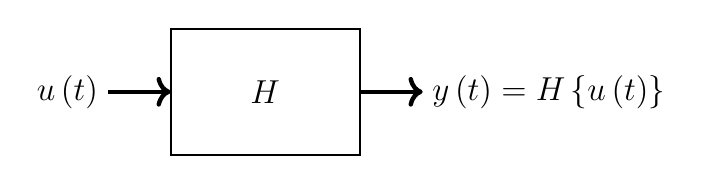
\begin{tikzpicture}[scale=0.8]
        \draw[thick] (0,0) rectangle (3, 2);
        \node at (1.5, 1) {{\large $H$}};
        \draw[ultra thick, ->] (-1, 1) -- (0, 1);
        \node[left] at (-1, 1) {{\large $u\lp t\rp$}};
        \draw[ultra thick, ->] (3, 1) -- (4, 1);
        \node[right] at (4, 1) {{\large $y\lp t\rp = H\lc u\lp t\rp\rc$}};
    \end{tikzpicture}
\caption{Schematic depiction of a system} \label{fig:ch1_system}
\end{figure}

Mathematically, one could think of a system as a map $H\ct{\bullet}$ that associates a set of input signals $U$ to a set of output signals $Y$, i.e.
\eqnwl{
    H\ct{\bullet}: U \mapsto Y
}

In this book, we will primarily talk about two different types of systems: continuous-time (CT) and discrete-time (DT). A CT system maps a set of CT input signals to a set of CT output signals, while a DT system maps DT input signals to DT output signals. In this book, we will focus primarily on linear time-invariant (LTI) systems. The current and next chapter deal with CT LTI  and DT LTI systems. 

\section{Why study linear time-invariant systems?}
The theroy of linear time-invariant (LTI) systems play and important role in engineering, and there are several reasons to study linear time-invariant systems.
\begin{enumerate}
    \item Most engineering systems that we encounter in nature can be well approximated by LTI system for understanding, analyzing and controlling their behavior. 
    \item The mathematical theory of linear time-invariant systems is well developed and there are lots of useful tools for dealing with these systems. This is not surprising because LTI systems are simpler to deal with than a non-linear time-variant system. 
\end{enumerate}

\section{Input-Output behavior of a system}

Consider a general system $H$ about which we know nothing about. We can interact with the system by applying some input and measure the corresponding output. To understand the behavior of the system, we could apply a set of inputs $U_{test} = \lc u_i \ct{t}\rc_{i=1}^N$ and observe the corresponding output $Y_{test} = \lc y_i \ct{t}\rc_{i=1}^N$, and tabulate the results. With the knowledge of these $N$ input-output (IO) pairs, what can we say about the output of the system for any arbitrary input $u\ct{t}$ that is not in $U_{test}$? In the case of a non-linear system, we cannot say anything; our knowledge of the system's IO characteristics are restricted to the set $U_{test}, Y_{test}$. But if we are told that the system is linear, then we know more about the IO characteristics of the system, beyond the known IO pairs $U_{test}, Y_{test}$. For a linear system, from the IO pairs, we also know the output of the system to any input of the form $u\ct{t} = \sum_{i=1}^N \alpha_iu_i\ct{t}$.
\[ y\ct{t} = H\ct{u\ct{t}} = H\ct{\sum_{i=1}^N\alpha_i u_i\ct{t}} = \sum_{i=1}^N \alpha_iH\ct{u_i\ct{t}} \]
\eqnwl{
    y\ct{t} = \sum_{i=1}^N \alpha_i y_i\ct{t}
    \label{ch3-linsys-io}
}

Eq. \ref{ch3-linsys-io} tells us that for a linear system, from $U_{test}, Y_{test}$, we also know the output of the system to any input that is a linear combination of the inputs in the set $U_{test}$.


% We will encounter several types of signals in our study of linear systems. This chapter discusses the different signals we will be used at some point during our discussion of linear systems. In this chapter we will cover both continuous-time and discrete-time signals; in fact this will be our general approach in all chapter, where we will cover both continuous-time and discrete-time concepts. 

% \section{Exponential Signals}
% \subsection{Continuos-time real exponential}
% A continuous-time real exponential signal is represented as the following,
% \[ x\left(t\right) = ae^{bt}, \,\,\, a, b \in \mb{R} \]
% \noindent where, $t$ is time, $a$ is the amplitude of the signal when $t = 0$, and $b$ the parameter indicate whether the $x\left(t\right)$ is an exponentially growing signal $\left(b > 0\right)$ or a exponentially decaying signal $\left(b < 0\right)$. 
% \begin{figure}[h]
% \centering
%     \includegraphics[width=0.95\textwidth]{figs/ch2-expsig.png}
% \caption{Continuous-time real exponential signals -- growing exponential on the left and a decaying exponential on the right.} \label{fig:ch2-expsig}
% \end{figure}
% When $b = 0$, then we get a constant signal $x\left(t\right) = a, \,\, \forall t$. The plot of $x\left(t\right)$ for different values of b is given in Fig. \ref{fig:ch2-expsig}.

% Exponential signals are often observed in physical systems. They play an important role in the analysis of linear time-invariant system. 

% \subsection{Discrete-time real exponential}
% A discrete-time real exponential signal is represented as,
% \[ x\dt{n} = b \times a^n, \quad \quad a, b \in \mb{R} \text{ and } n \in \mb{Z} \]
% This signal represents a growing exponential if $a > 1$, and its a decaying exponential if $0 < a < 1$; these are shown in Fig \ref{fig:ch2_discexpsig}. 

% \begin{figure}[h]
% \centering
%     \includegraphics[width=0.95\textwidth]{figs/ch2-discexpsig.png}
% \caption{Continuous-time real exponential signals -- growing exponential on the left and a decaying exponential on the right.} \label{fig:ch2_discexpsig}
% \end{figure}

% \begin{problem*}[frametitle=Discrete-time exponential signals]
%     \begin{enumerate}
%         \item What does $a^n$ look like when: (a) $-1 < a < 0$; and (b) $a < -1$?
%     \end{enumerate}
% \end{problem*}

% \section{Sinusoidal Signals}
% \subsection{Continuous-time sinusoids}
% The general form of a continuous-time sinusoidal signals is given by the following,
% \[ x\left(t\right) = A\sin\left(\omega t + \phi\right), \]
% \noindent where $A$ is the amplitude of the sinusoidal signal, $\omega$ is the angular frequency (radian per sec), and $\phi$ is the phase angle in radians. The sinusoid is an example of a periodic signal with the fundamental period $T = \frac{2\pi}{\omega}$ (Fig. \ref{fig:ch2_sine}).
% \begin{figure}[h]
% \centering
%     \includegraphics[width=\textwidth]{figs/ch2-sine.png}
% \caption{Continuous-time real exponential signals -- growing exponential on the left and a decaying exponential on the right.} ch2-\label{fig:ch2_sine}
% \end{figure}

% \begin{problem*}[frametitle=Discrete-time exponential signals]
%     Please verify that $T$ is the fundamental period of $x\ct{t} = A\sin\ct{\omega t + \phi}$.
% \end{problem*}

% The exponential signal was earlier introduced as the real exponential, as the parameters of the signal are real numbers. In fact a more general form of exponential singals is the complex exponential, where the parameters are allowed to be complex numbers. A complex exponential can be witten as,
% \[ x\left(t\right) = Ae^{bt}, \, t \in \mathbb{R}, \,\, A, b \in \mathbb{C} \]

% Consider a complex exponential signal $e^{j\omega t}$. This can written as the following using the \textit{Euler identity}.
% \[ e^{j\omega t} = \cos\left(\omega t\right) + j\sin\left(\omega t\right) \]

% Thus a continuous-time sinusoid can be written as the real or imaginary part of the complex exponential.
% \[ \cos\left(\omega t + \phi\right) = \Re\left(e^{j\omega t + \phi}\right) \]
% \[ \sin\left(\omega t + \phi\right) = \Im\left(e^{j\omega t + \phi}\right) \]

% Another representation of sinusoidal signals in terms of complex exponential is the following,
% \[ \cos\left(\omega t + \phi\right) = \frac{e^{\left(j\omega t + \phi\right)} + e^{-\left(j\omega t + \phi\right)}}{2} \]
% \[ \sin\left(\omega t + \phi\right) = \frac{e^{\left(j\omega t + \phi\right)} - e^{-\left(j\omega t + \phi\right)}}{2j} \]

% \subsection{Discrete-time sinusoids}
% The discrete-time equivalent of the sinusoids are represented as the following,
% \[ x\dt{n} = A \sin \ct{\Omega n + \phi} \]
% \noindent where, $A$ is the amplitude of the sinusoid, $\Omega$ is the discrete frequency (radians per sample), and $\phi$ is the phase. A plot of a discrete-time sinusoid is shown in Fig. \ref{fig:ch2-discsine}.
% \begin{figure}[h]
% \centering
%     \includegraphics[width=\textwidth]{figs/ch2-discsine.png}
% \caption{Continuous-time real exponential signals -- growing exponential on the left and a decaying exponential on the right.} \label{fig:ch2-discsine}
% \end{figure}

% The period of $x\dt{n}$ is $N = k\frac{2\pi}{\Omega}$, where $k \in \mb{Z}$ such that $N \in \mb{Z}$. The discrete-time sinusoid has several features that are quite different to that of the continuous-time sinusoid. The following problems bring out some of these features.

% \begin{problem*}[frametitle=Discrete-time sinusoidal signals]
%     \begin{enumerate}
%         \item Please verify that $N = k\frac{2\pi}{\Omega}$ ($k \in \mb{Z}$ such that $N \in \mb{Z}$) is the period of $\sin \ct{\Omega n + \phi}$.
%         \item Prove that the discrete frequency $\Omega$ can only take values between $0 \leq \Omega < \pi$. 
%         \item There are some sinusoidal signals that are not periodic. Verify that $\sin \ct{n}$ is not periodic. 
%     \end{enumerate}
% \end{problem*}

% \section{Exponential Sinusoidal Signals}
% A natural extension of the representation of sinusoids in terms of complex exponentials is to combine the real and complex exponentials, which results in the exponential sinusoidal signals. A exponentially weighted sinusoid is obtained by multiplying a sinusoidal signal $\ct{\sin\ct{\omega t + \phi}}$ by a real exponential signal $\ct{e^{\alpha t}}$,
% \[ x\ct{t} = Ae^{\alpha t}\sin\ct{\omega t + \phi} \]

% \begin{figure}[h]
% \centering
%     \includegraphics[width=\textwidth]{figs/ch2-expsine.png}
% \caption{Exponential continuous-time sinusoidal signals -- growing exponential on the left and a decaying exponential on the right.} \label{fig:ch2-expsine}
% \end{figure}

% \noindent $x\ct{t}$ can be represented using complex exponentials as,
% \[ x\ct{t} = Ae^{\alpha t}\sin\ct{\omega t + \phi} = A\frac{e^{\ct{\alpha + j\omega}t} - e^{-\ct{\alpha + j\omega}t}}{2j} = Ae^{\alpha t}\frac{e^{j\omega t} - e^{-j\omega t}}{2j} \]

% \begin{problem*}[frametitle=Discrete-time exponential sinusoidal signals]
%     Write down the expression for a discrete-time exponential sinusoidal signal. Explain how the different parameters affect the nature of the signal.
% \end{problem*}

% \section{Impulse function}
% \subsection{Continuous-time impulse function}
% The first and most important fact to remember about the impulse function is that it is not an ordinary function. The impulse function $\delta\left(t\right)$, also know as the Dirac delta function, is not characterized by the exact values it takes for the different values of its argument, rather it is characterized by the following property,
% \[ \int_{a}^{b}\delta\left(t\right)dt = 
% \begin{cases}
%     1, & 0 \in \left[a, b\right] \\
%     0, & \mathrm{Otherwise}
% \end{cases}
% \]

% This property tells us that the impulse function is concentrated around the origin $t = 0$. 

% A useful property of the impulse function is that \textit{\textbf{sifting property}}, For any ordinary function $f\left(t\right)$, which is continuous at $t = t_0$,
% \[ \int_{-\infty}^{\infty}f\left(t - t_0\right)\delta\left(t\right)dt = f\left(t_0\right) \]

% One way to think of the impulse function in terms of ordinary functions is to see it a limit of a sequence or family of functions. One sequence that is commonly encountered in books on signals and systems is the following,
% \[ g_{n}\left(t\right) = 
% \begin{cases}
% n, & -\frac{1}{2n} \leq t \leq \frac{1}{2n} \\
% 0, & \mathrm{Otherwise}
% \end{cases}
% \]

% This is a rectangular function that grows taller as $n \to \infty$. Now, lets take $g_{n}\left(t\right)$ and apply it on an ordinary function $f\ct{t}$,
% \[ \int_{-\infty}^{\infty}g_{n}\ct{t}f\ct{t}dt = \int_{-\frac{1}{2n}}^{\frac{1}{2n}}nf\ct{t}dt = f_n \]

% And,
% \[ \lim_{n\to\infty}\int_{-\infty}^{\infty}g_{n}\ct{t}f\ct{t}dt = \lim_{n\to\infty}f_n = f\ct{0} \]

% This is demonstrated in Fig. \ref{fig:ch2-impsifseq}.

% \begin{figure}[h]
% \centering
%     \includegraphics[width=\textwidth]{figs/ch2-impulsesift.png}
%     \caption{Viewing the impulse function as a limit of a sequence of rectangular pulses.}
%     \label{fig:ch2-impsifseq}
% \end{figure}

% \subsection{Discrete-time impulse function}
% The discrete-time impulse function is theoretically a much simpler function deal with. The discrete-time impulse function is defined as,
% \[ \delta\dt{n} = 
% \begin{cases}
%     1, & n = 0 \\
%     0, & n \neq 0
% \end{cases}
% \]

% \begin{figure}[h]
% \centering
%     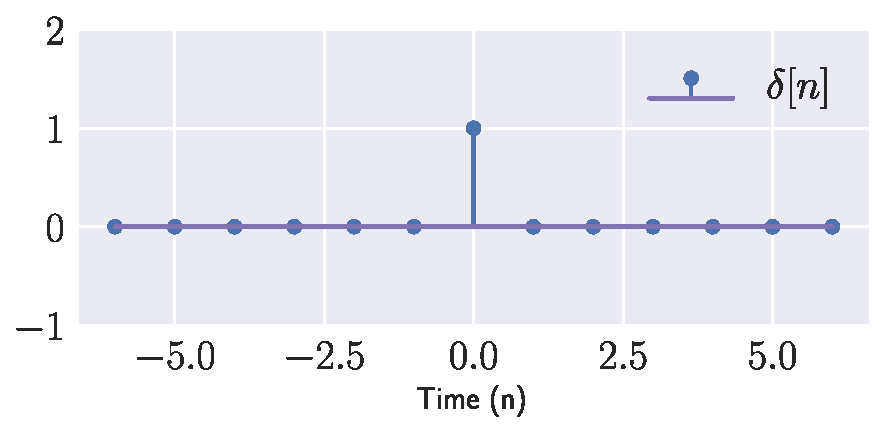
\includegraphics[width=0.65\textwidth]{figs/ch2-impulse-disc.eps}
%     \caption{Discrete-time impulse signal.}
%     \label{fig:ch2-impdisc}
% \end{figure}

% \subsection{Step Function}
% \subsection{Continuous-time step function}
% The step function is defined using the impulse function as the following,
% \[ 1\left(t\right) = \int_{-\infty}^{t}\delta\left(\tau\right)d\tau = 
% \begin{cases}
%     1, & t > 0 \\
%     0, & t < 0 \\
%     \frac{1}{2}, & t = 0
% \end{cases} 
% \]

% \noindent This function has a step discontinuity at $t = 0$.

% \begin{figure}[h]
% \centering
%     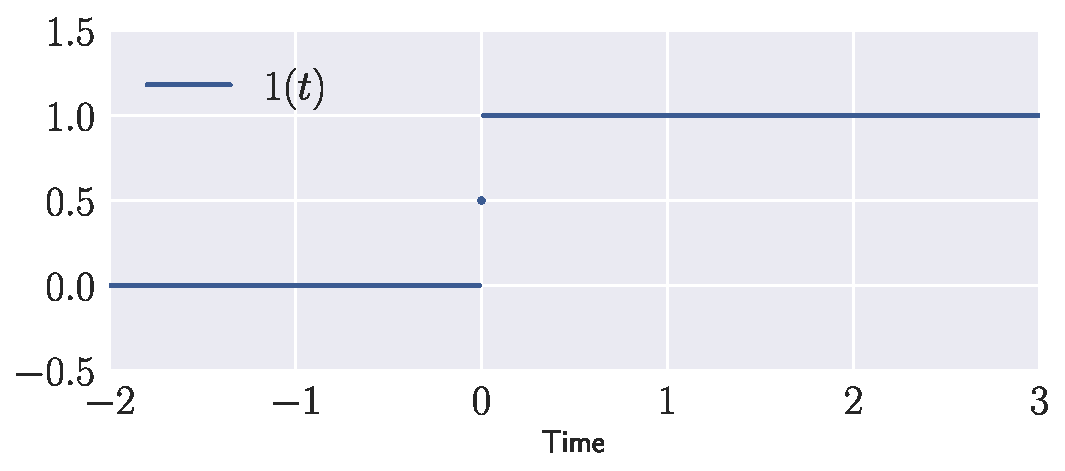
\includegraphics[width=0.7\textwidth]{figs/ch2-step-cont.eps}
%     \caption{Viewing the impulse function as a limit of a sequence of rectangular pulses.}
%     \label{fig:ch2-stepcont}
% \end{figure}

% \begin{problem*}[frametitle=Discrete-time step signal]
%     What would be definition of a discrete-time step function? How would you represent the discrete-time step function in terms of the discrete-time impulse function. 
% \end{problem*}
% % -*- root: ../lsnotess.tex -*-

\chapter{Discrete-time Linear Time-Invariant systems}

% % \begin{chapquote}{Author's name, \textit{Source of this quote}}
% % ``This is a quote and I don't know who said this.''
% % \end{chapquote}

% We will encounter several types of signals in our study of linear systems. This chapter discusses the different signals we will be used at some point during our discussion of linear systems. In this chapter we will cover both continuous-time and discrete-time signals; in fact this will be our general approach in all chapter, where we will cover both continuous-time and discrete-time concepts. 

% \section{Exponential Signals}
% \subsection{Continuos-time real exponential}
% A continuous-time real exponential signal is represented as the following,
% \[ x\left(t\right) = ae^{bt}, \,\,\, a, b \in \mb{R} \]
% \noindent where, $t$ is time, $a$ is the amplitude of the signal when $t = 0$, and $b$ the parameter indicate whether the $x\left(t\right)$ is an exponentially growing signal $\left(b > 0\right)$ or a exponentially decaying signal $\left(b < 0\right)$. 
% \begin{figure}[h]
% \centering
%     \includegraphics[width=0.95\textwidth]{figs/ch2-expsig.png}
% \caption{Continuous-time real exponential signals -- growing exponential on the left and a decaying exponential on the right.} \label{fig:ch2-expsig}
% \end{figure}
% When $b = 0$, then we get a constant signal $x\left(t\right) = a, \,\, \forall t$. The plot of $x\left(t\right)$ for different values of b is given in Fig. \ref{fig:ch2-expsig}.

% Exponential signals are often observed in physical systems. They play an important role in the analysis of linear time-invariant system. 

% \subsection{Discrete-time real exponential}
% A discrete-time real exponential signal is represented as,
% \[ x\dt{n} = b \times a^n, \quad \quad a, b \in \mb{R} \text{ and } n \in \mb{Z} \]
% This signal represents a growing exponential if $a > 1$, and its a decaying exponential if $0 < a < 1$; these are shown in Fig \ref{fig:ch2_discexpsig}. 

% \begin{figure}[h]
% \centering
%     \includegraphics[width=0.95\textwidth]{figs/ch2-discexpsig.png}
% \caption{Continuous-time real exponential signals -- growing exponential on the left and a decaying exponential on the right.} \label{fig:ch2_discexpsig}
% \end{figure}

% \begin{problem*}[frametitle=Discrete-time exponential signals]
%     \begin{enumerate}
%         \item What does $a^n$ look like when: (a) $-1 < a < 0$; and (b) $a < -1$?
%     \end{enumerate}
% \end{problem*}

% \section{Sinusoidal Signals}
% \subsection{Continuous-time sinusoids}
% The general form of a continuous-time sinusoidal signals is given by the following,
% \[ x\left(t\right) = A\sin\left(\omega t + \phi\right), \]
% \noindent where $A$ is the amplitude of the sinusoidal signal, $\omega$ is the angular frequency (radian per sec), and $\phi$ is the phase angle in radians. The sinusoid is an example of a periodic signal with the fundamental period $T = \frac{2\pi}{\omega}$ (Fig. \ref{fig:ch2_sine}).
% \begin{figure}[h]
% \centering
%     \includegraphics[width=\textwidth]{figs/ch2-sine.png}
% \caption{Continuous-time real exponential signals -- growing exponential on the left and a decaying exponential on the right.} ch2-\label{fig:ch2_sine}
% \end{figure}

% \begin{problem*}[frametitle=Discrete-time exponential signals]
%     Please verify that $T$ is the fundamental period of $x\ct{t} = A\sin\ct{\omega t + \phi}$.
% \end{problem*}

% The exponential signal was earlier introduced as the real exponential, as the parameters of the signal are real numbers. In fact a more general form of exponential singals is the complex exponential, where the parameters are allowed to be complex numbers. A complex exponential can be witten as,
% \[ x\left(t\right) = Ae^{bt}, \, t \in \mathbb{R}, \,\, A, b \in \mathbb{C} \]

% Consider a complex exponential signal $e^{j\omega t}$. This can written as the following using the \textit{Euler identity}.
% \[ e^{j\omega t} = \cos\left(\omega t\right) + j\sin\left(\omega t\right) \]

% Thus a continuous-time sinusoid can be written as the real or imaginary part of the complex exponential.
% \[ \cos\left(\omega t + \phi\right) = \Re\left(e^{j\omega t + \phi}\right) \]
% \[ \sin\left(\omega t + \phi\right) = \Im\left(e^{j\omega t + \phi}\right) \]

% Another representation of sinusoidal signals in terms of complex exponential is the following,
% \[ \cos\left(\omega t + \phi\right) = \frac{e^{\left(j\omega t + \phi\right)} + e^{-\left(j\omega t + \phi\right)}}{2} \]
% \[ \sin\left(\omega t + \phi\right) = \frac{e^{\left(j\omega t + \phi\right)} - e^{-\left(j\omega t + \phi\right)}}{2j} \]

% \subsection{Discrete-time sinusoids}
% The discrete-time equivalent of the sinusoids are represented as the following,
% \[ x\dt{n} = A \sin \ct{\Omega n + \phi} \]
% \noindent where, $A$ is the amplitude of the sinusoid, $\Omega$ is the discrete frequency (radians per sample), and $\phi$ is the phase. A plot of a discrete-time sinusoid is shown in Fig. \ref{fig:ch2-discsine}.
% \begin{figure}[h]
% \centering
%     \includegraphics[width=\textwidth]{figs/ch2-discsine.png}
% \caption{Continuous-time real exponential signals -- growing exponential on the left and a decaying exponential on the right.} \label{fig:ch2-discsine}
% \end{figure}

% The period of $x\dt{n}$ is $N = k\frac{2\pi}{\Omega}$, where $k \in \mb{Z}$ such that $N \in \mb{Z}$. The discrete-time sinusoid has several features that are quite different to that of the continuous-time sinusoid. The following problems bring out some of these features.

% \begin{problem*}[frametitle=Discrete-time sinusoidal signals]
%     \begin{enumerate}
%         \item Please verify that $N = k\frac{2\pi}{\Omega}$ ($k \in \mb{Z}$ such that $N \in \mb{Z}$) is the period of $\sin \ct{\Omega n + \phi}$.
%         \item Prove that the discrete frequency $\Omega$ can only take values between $0 \leq \Omega < \pi$. 
%         \item There are some sinusoidal signals that are not periodic. Verify that $\sin \ct{n}$ is not periodic. 
%     \end{enumerate}
% \end{problem*}

% \section{Exponential Sinusoidal Signals}
% A natural extension of the representation of sinusoids in terms of complex exponentials is to combine the real and complex exponentials, which results in the exponential sinusoidal signals. A exponentially weighted sinusoid is obtained by multiplying a sinusoidal signal $\ct{\sin\ct{\omega t + \phi}}$ by a real exponential signal $\ct{e^{\alpha t}}$,
% \[ x\ct{t} = Ae^{\alpha t}\sin\ct{\omega t + \phi} \]

% \begin{figure}[h]
% \centering
%     \includegraphics[width=\textwidth]{figs/ch2-expsine.png}
% \caption{Exponential continuous-time sinusoidal signals -- growing exponential on the left and a decaying exponential on the right.} \label{fig:ch2-expsine}
% \end{figure}

% \noindent $x\ct{t}$ can be represented using complex exponentials as,
% \[ x\ct{t} = Ae^{\alpha t}\sin\ct{\omega t + \phi} = A\frac{e^{\ct{\alpha + j\omega}t} - e^{-\ct{\alpha + j\omega}t}}{2j} = Ae^{\alpha t}\frac{e^{j\omega t} - e^{-j\omega t}}{2j} \]

% \begin{problem*}[frametitle=Discrete-time exponential sinusoidal signals]
%     Write down the expression for a discrete-time exponential sinusoidal signal. Explain how the different parameters affect the nature of the signal.
% \end{problem*}

% \section{Impulse function}
% \subsection{Continuous-time impulse function}
% The first and most important fact to remember about the impulse function is that it is not an ordinary function. The impulse function $\delta\left(t\right)$, also know as the Dirac delta function, is not characterized by the exact values it takes for the different values of its argument, rather it is characterized by the following property,
% \[ \int_{a}^{b}\delta\left(t\right)dt = 
% \begin{cases}
%     1, & 0 \in \left[a, b\right] \\
%     0, & \mathrm{Otherwise}
% \end{cases}
% \]

% This property tells us that the impulse function is concentrated around the origin $t = 0$. 

% A useful property of the impulse function is that \textit{\textbf{sifting property}}, For any ordinary function $f\left(t\right)$, which is continuous at $t = t_0$,
% \[ \int_{-\infty}^{\infty}f\left(t - t_0\right)\delta\left(t\right)dt = f\left(t_0\right) \]

% One way to think of the impulse function in terms of ordinary functions is to see it a limit of a sequence or family of functions. One sequence that is commonly encountered in books on signals and systems is the following,
% \[ g_{n}\left(t\right) = 
% \begin{cases}
% n, & -\frac{1}{2n} \leq t \leq \frac{1}{2n} \\
% 0, & \mathrm{Otherwise}
% \end{cases}
% \]

% This is a rectangular function that grows taller as $n \to \infty$. Now, lets take $g_{n}\left(t\right)$ and apply it on an ordinary function $f\ct{t}$,
% \[ \int_{-\infty}^{\infty}g_{n}\ct{t}f\ct{t}dt = \int_{-\frac{1}{2n}}^{\frac{1}{2n}}nf\ct{t}dt = f_n \]

% And,
% \[ \lim_{n\to\infty}\int_{-\infty}^{\infty}g_{n}\ct{t}f\ct{t}dt = \lim_{n\to\infty}f_n = f\ct{0} \]

% This is demonstrated in Fig. \ref{fig:ch2-impsifseq}.

% \begin{figure}[h]
% \centering
%     \includegraphics[width=\textwidth]{figs/ch2-impulsesift.png}
%     \caption{Viewing the impulse function as a limit of a sequence of rectangular pulses.}
%     \label{fig:ch2-impsifseq}
% \end{figure}

% \subsection{Discrete-time impulse function}
% The discrete-time impulse function is theoretically a much simpler function deal with. The discrete-time impulse function is defined as,
% \[ \delta\dt{n} = 
% \begin{cases}
%     1, & n = 0 \\
%     0, & n \neq 0
% \end{cases}
% \]

% \begin{figure}[h]
% \centering
%     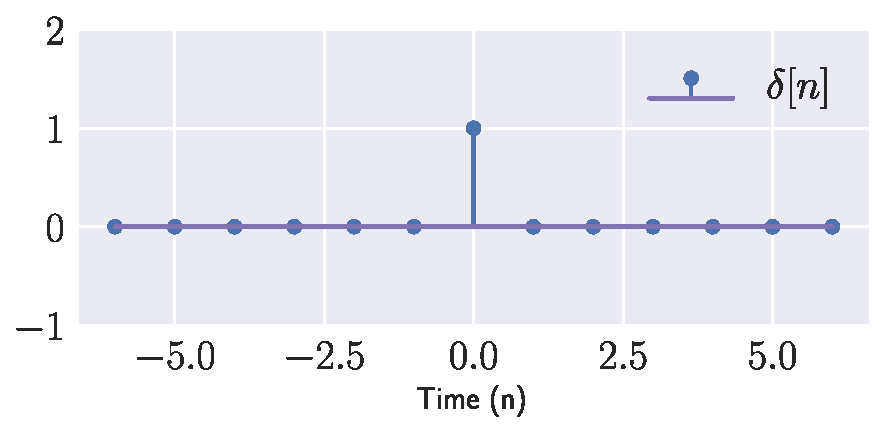
\includegraphics[width=0.65\textwidth]{figs/ch2-impulse-disc.eps}
%     \caption{Discrete-time impulse signal.}
%     \label{fig:ch2-impdisc}
% \end{figure}

% \subsection{Step Function}
% \subsection{Continuous-time step function}
% The step function is defined using the impulse function as the following,
% \[ 1\left(t\right) = \int_{-\infty}^{t}\delta\left(\tau\right)d\tau = 
% \begin{cases}
%     1, & t > 0 \\
%     0, & t < 0 \\
%     \frac{1}{2}, & t = 0
% \end{cases} 
% \]

% \noindent This function has a step discontinuity at $t = 0$.

% \begin{figure}[h]
% \centering
%     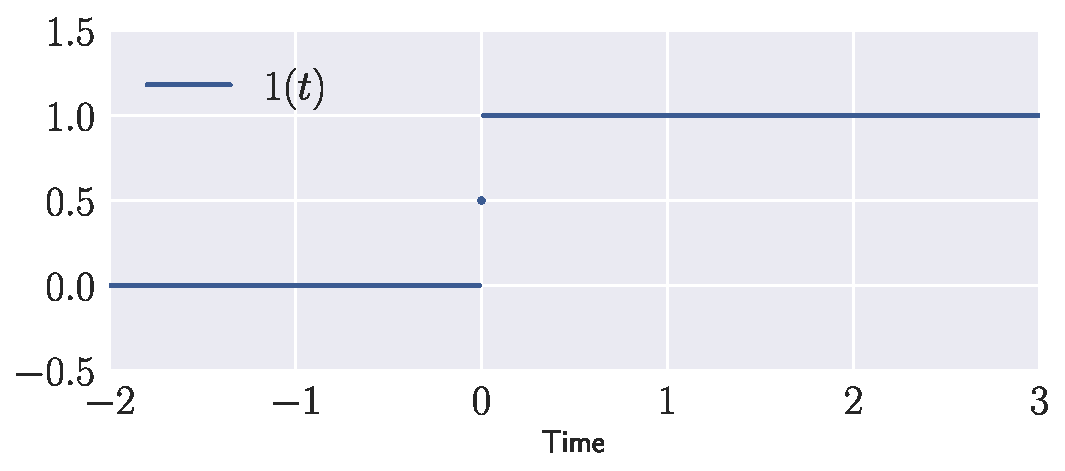
\includegraphics[width=0.7\textwidth]{figs/ch2-step-cont.eps}
%     \caption{Viewing the impulse function as a limit of a sequence of rectangular pulses.}
%     \label{fig:ch2-stepcont}
% \end{figure}

% \begin{problem*}[frametitle=Discrete-time step signal]
%     What would be definition of a discrete-time step function? How would you represent the discrete-time step function in terms of the discrete-time impulse function. 
% \end{problem*}
% -*- root: ../lsnotes.tex -*-

\chapter{Problems}

\begin{chapquote}{Confucius, \textit{}}
``I hear and I forget. I see and I remember. I do and I understand.''
\end{chapquote}

\section{Linear Time-Invariant (LTI) Systems}
\begin{enumerate}
    \item Prove that for a memoryless LTI system the output is a scaled version of the input. Is this also true for:
    \begin{enumerate*}
         \item a linear time-variant system; and 
         \item a non-linear system?
     \end{enumerate*} 
    Explain your answer.

\end{enumerate}

\end{document}
